%% This is file `elsarticle-template-1a-num.tex',
%%
%% Copyright 2009 Elsevier Ltd
%%
%% This file is part of the 'Elsarticle Bundle'.
%% ---------------------------------------------
%%
%% It may be distributed under the conditions of the LaTeX Project Public
%% License, either version 1.2 of this license or (at your option) any
%% later version.  The latest version of this license is in
%%    http://www.latex-project.org/lppl.txt
%% and version 1.2 or later is part of all distributions of LaTeX
%% version 1999/12/01 or later.
%%
%% The list of all files belonging to the 'Elsarticle Bundle' is
%% given in the file `manifest.txt'.
%%
%% Template article for Elsevier's document class `elsarticle'
%% with numbered style bibliographic references
%%
%% $Id: elsarticle-template-1a-num.tex 151 2009-10-08 05:18:25Z rishi $
%% $URL: http://lenova.river-valley.com/svn/elsbst/trunk/elsarticle-template-1a-num.tex $
%%
\documentclass[preprint,12pt]{elsarticle}

%% Use the option review to obtain double line spacing
%% \documentclass[preprint,review,12pt]{elsarticle}

%% Use the options 1p,twocolumn; 3p; 3p,twocolumn; 5p; or 5p,twocolumn
%% for a journal layout:
%% \documentclass[final,1p,times]{elsarticle}
%% \documentclass[final,1p,times,twocolumn]{elsarticle}
%% \documentclass[final,3p,times]{elsarticle}
%% \documentclass[final,3p,times,twocolumn]{elsarticle}
%% \documentclass[final,5p,times]{elsarticle}
%% \documentclass[final,5p,times,twocolumn]{elsarticle}

%% if you use PostScript figures in your article
%% use the graphics package for simple commands
%% \usepackage{graphics}
%% or use the graphicx package for more complicated commands
\usepackage{graphicx}
%% or use the epsfig package if you prefer to use the old commands
%% \usepackage{epsfig}

%% The amssymb package provides various useful mathematical symbols
\usepackage{amssymb}
%% The amsthm package provides extended theorem environments
%% \usepackage{amsthm}

%% The lineno packages adds line numbers. Start line numbering with
%% \begin{linenumbers}, end it with \end{linenumbers}. Or switch it on
%% for the whole article with \linenumbers after \end{frontmatter}.
%% \usepackage{lineno}

%% natbib.sty is loaded by default. However, natbib options can be
%% provided with \biboptions{...} command. Following options are
%% valid:

%%   round  -  round parentheses are used (default)
%%   square -  square brackets are used   [option]
%%   curly  -  curly braces are used      {option}
%%   angle  -  angle brackets are used    <option>
%%   semicolon  -  multiple citations separated by semi-colon
%%   colon  - same as semicolon, an earlier confusion
%%   comma  -  separated by comma
%%   numbers-  selects numerical citations
%%   super  -  numerical citations as superscripts
%%   sort   -  sorts multiple citations according to order in ref. list
%%   sort&compress   -  like sort, but also compresses numerical citations
%%   compress - compresses without sorting
%%
%% \biboptions{comma,round}

% \biboptions{}


\journal{Nuclear Physics B}

\begin{document}

\begin{frontmatter}

%% Title, authors and addresses

%% use the tnoteref command within \title for footnotes;
%% use the tnotetext command for the associated footnote;
%% use the fnref command within \author or \address for footnotes;
%% use the fntext command for the associated footnote;
%% use the corref command within \author for corresponding author footnotes;
%% use the cortext command for the associated footnote;
%% use the ead command for the email address,
%% and the form \ead[url] for the home page:
%%
%% \title{Title\tnoteref{label1}}
%% \tnotetext[label1]{}
%% \author{Name\corref{cor1}\fnref{label2}}
%% \ead{email address}
%% \ead[url]{home page}
%% \fntext[label2]{}
%% \cortext[cor1]{}
%% \address{Address\fnref{label3}}
%% \fntext[label3]{}

\title{This is my first paper}

%% use optional labels to link authors explicitly to addresses:
%% \author[label1,label2]{<author name>}
%% \address[label1]{<address>}
%% \address[label2]{<address>}

\author{NatRiskChnge}

\address{}

\begin{abstract}
%% Text of abstract
Following an unusual heavy precipitation of 105 mm on 29th May 2016 within ~4 hours, intense rainfall events in southern Germany led to severe flash floods and debris flows in several municipalities in the German federal state of Baden-W{\"u}rttemberg. Particularly the south-western German town of Braunsbach witnessed flood outburst with massive amounts of rubbles and muddy sediments. The flash flood, as the combination of surging water with 42,000 m3 of sediment, was responsible for smashing numerous buildings, cars, and town facilities; leaving residents with damages and losses. The high concentrations of sediment are attributed to the 48 landslides, river bank erosion, and remarkable river bed incision along the Orlacher Bach.  While this material included large rock debris, soil, woody debris, concrete, asphalt and different artificial construction-derived residues, it is estimated that about 80\% of this (\i.e. 33,600 m3) were non-organic natural sediments (i.e. either suspended sediment or bedload). If the event and study catchment are compared with similar past events and with the regional catchments it could be ascertained that the event lies well above the 95th percentile. The present study gives the meteorological overview and hydro-geological assessment of the event.
\end{abstract}

\begin{keyword}
%% keywords here, in the form: keyword \sep keyword

%% MSC codes here, in the form: \MSC code \sep code
%% or \MSC[2008] code \sep code (2000 is the default)

\end{keyword}

\end{frontmatter}

%%
%% Start line numbering here if you want
%%
% \linenumbers

%% main text
\section{Introduction}

Impacts of floods increase along with the growth of the population and the economy. They are the most devastating natural hazard not only in Europe but also worldwide the main cause of natural disaster-related life loss (Jonkman, 2005).

\begin{equation}
R=\frac{\sum_{i} Q_{i} x_i}{\sum_{i} Q_i}
\end{equation}

\section{Study Area}

Braunsbach is a village of 2518 inhabitants, located in the northeastern part of Baden-W{\"u}rttemberg, belonging to the administrative district Schw{\"a}bisch Hall next to the district of Hohenlohekreis (south Germany) (Figure 1a). The topography is characterized by hilly terrain with an elevation ranging from ~150 m to 580 m above sea level (Figure 1b).

\section{Methodology}

\subsection{Rainfall}

Weather radars provide rainfall estimates with spatial and temporal resolution unmatched by traditional rain gauge networks, making a valuable tool in flash-flood monitoring and analysis (Borga et al., 2007). Hence, the 5-min DX product of the T�rkheim radar of the German Weather Service (DWD) from 27th May to 30th May 2016 was used in this work. 

\begin{figure}
  \centering
    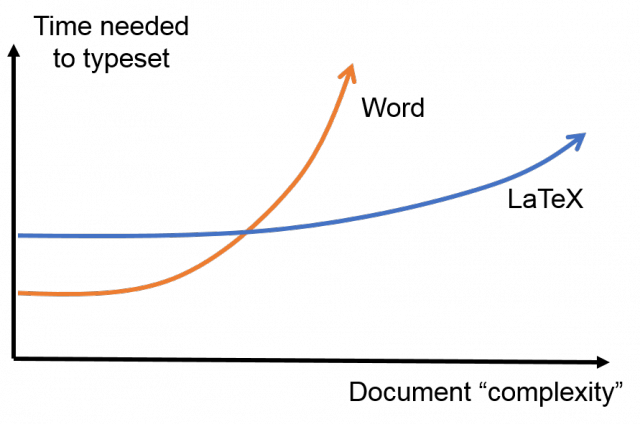
\includegraphics[width=10cm]{myplot1}
  \caption{Time vs Complexity}
\end{figure}

\subsection{Estimation of the material detached from the catchment as landslides}

\begin{tabular}{ l | c | r }
  1 & 2 & 3 \\ \hline
  4 & 5 & 6 \\
  7 & 8 & 9 \\
\end{tabular}


\begin{tabular}{ l | c | r }
\hline
  left & 2 & 3 \\ \hline
  left & center & right \\
  7 & 8 & 9 \\
\hline
\end{tabular}

\begin{table}[]
\centering

\label{my-label}
\begin{tabular}{lllll}
category & 1 & 2 & 3 & 4 \\ \hline
a        &   &   &   &   \\
b        &   &   &   &   \\
c        &   &   &   &  
\end{tabular}
\caption{My caption}
\end{table}

\begin{table}[]
\centering
\caption{My caption}
\label{my-label}
\begin{tabular}{lllll}
\hline
cat & A   & B   & C   & D   \\ \hline
1   & 0.5 & 0.5 & 0.5 & 0.5 \\
2   & 0.5 & 0.5 & 0.5 & 0.5 \\
3   & 0.5 & 0.5 & 0.5 & 0.5 \\ \hline
\end{tabular}
\end{table}

\begin{equation}
\sum x \frac{1}{2} 
\end{equation}



%% The Appendices part is started with the command \appendix;
%% appendix sections are then done as normal sections
%% \appendix

%% \section{}
%% \label{}

%% References
%%
%% Following citation commands can be used in the body text:
%% Usage of \cite is as follows:
%%   \cite{key}          ==>>  [#]
%%   \cite[chap. 2]{key} ==>>  [#, chap. 2]
%%   \citet{key}         ==>>  Author [#]

%% References with bibTeX database:

\bibliographystyle{model1a-num-names}
\bibliography{<your-bib-database>}

%% Authors are advised to submit their bibtex database files. They are
%% requested to list a bibtex style file in the manuscript if they do
%% not want to use model1a-num-names.bst.

%% References without bibTeX database:

% \begin{thebibliography}{00}

%% \bibitem must have the following form:
%%   \bibitem{key}...
%%

% \bibitem{}

% \end{thebibliography}


\end{document}

%%
%% End of file `elsarticle-template-1a-num.tex'.
